\chapter{Analysis}

\begin{chapterabstract}
A comprehensive evaluation of existing solutions, identification of key features and limitations, and outlining of the specifications for the proposed solution.
\end{chapterabstract}

Product configurators can be implemented in various ways, and the design of the tool itself determines the types of products that can be customized using the tool later on. The number of unique configurations of a product that the tool can create is called the solution space. The size of the solution space is determined by two factors: the number of customizable attributes and the achievable values of each attribute. \cite{Huiwen2018} A relevant study examined the solution spaces of these toolkits and proposed an evaluation model that enables the categorization and assessment of various implementation approaches. Based on the target outcome and the guidance provided by the tool, the following mechanisms are specified: \cite{Hermans2012}

\begin{definition}[Veneer]
Customization by adding a visual decorative layer. (e.g., printing, engraving, etching)
\end{definition}
\begin{definition}[Modularity]
Customization by combining modules or components.
\end{definition}
\begin{definition}[Parametric]
Customization by changing the parameter values of parts.
\end{definition}
\begin{definition}[Generative]
Customization using code and scripting to synthesize the final form of the product.
\end{definition}

There are often some common characteristics among configuration tools with different mechanisms; however, the main focus of this thesis is on toolkits that primarily employ modularity mechanisms.


%---------------------------------------------------------------
\section{Existing solutions}
%---------------------------------------------------------------
% - - - - - - - - - - - - - - - - - - - - - - - - - - - - - - -
\subsection{Applications of product configurators}
% - - - - - - - - - - - - - - - - - - - - - - - - - - - - - - -

Many companies are integrating product configurators into their sales strategies across multiple industries, such as automotive, fashion, furniture, housing, etc. These configurators serve as the main or supplementary sales tools for these businesses.

The Configurator Database Project by cyLEDGE MEDIA aims to catalog these web-based configuration tools. The 2017/2018 report tracked 1250 deployments of these tools; however, the true count will be significantly higher since the database only includes the most frequently visited applications. \cite{cyLEDGE2018}

An analysis of the 100 most viewed configurators  from May 2020 to May 2021 was performed in the Configurator Database Project in a study that examined the shared characteristics of these configurations \cite{Blazek2023}. The results of some of the relevant characteristics and design choices that the study has analyzed are presented in this section:
\begin{description}
    \item[Responsive design:] 75.3\% of examined tools had responsive design (the design adapted to the viewport of the device).
    \item[Navigation:] 17.5\% of configurators had linear predefined navigation (meaning the configuration had to follow a specified sequence), whereas the 82.5\% majority of tools had open navigation (user has the flexibility to configure the product in any order).
    \item[Visualization:] 79.4\% of tools utilized photorealistic visualization (as opposed to illustrations or no visualization); however, the study acknowledges that there were significant variations depending on the industries in which the configurator is utilized.
    \item[Data transfer:] The mean network data size transferred for 3D configurator was 35.6~MB.
    \item[Configuration options:] 60.8\% of configurators offered more than ten customizable attributes.
    \item[Purchase capability:] Given that car brands typically do not directly sell their cars online, they were excluded from the analysis of this particular characteristic. Without vehicle configurators, 70.5\% of the configurators could complete an online purchase of the configured product.
    \item[Price calculation:] 56.7\% of the configurators were able to instantly reflect the changes made to the configuration in the displayed price.
\end{description}

Another article \cite{Leitner2014} also used The Configurator Database Project to analyze common design elements. They identified several key designs that were prevalent in the majority of configurators analyzed. The following key insights of commonly used designs from the article are relevant to this thesis:
\begin{itemize}[label=\rectanglebullet]
    \item At the end of the configuration process, a summary of selected options is presented.
    \item To present the products that can be configured, detailed images are used.
    \item If the configurator has linear predefined navigation, the navigation information is presented on a horizontal plane.
    \item Navigation bar is visible.
    \item Price and order button is clearly visible and available for completion purposes.
    \item Prices of the components are accessible in all phases of the configuration.
    \item Logo of the business is displayed prominently.
\end{itemize}

The previous paragraphs discussed general trends among all product configurators of all kinds. As part of the analysis in this chapter, it is essential also to examine existing modular 3D product configurators. 

Due to the large number of existing applications, it is not within the scope of this work to perform an exhaustive analysis. Instead, this section will focus on a select group of three applications. These have been selected based on a combination of factors such as their popularity, functionality, and importance in the context of a modular product configuration. This selection is intended to provide insightful examples that highlight different approaches, rather than being representative of the entire domain.

\noindent The main aspects under consideration are as follows:\nopagebreak
\begin{itemize}[label=\rectanglebullet]
    \item \textbf{Navigation:} How does the user navigate in the application during the configuration process?
    \item \textbf{Visualization style:} How is the product visualized within the configuration process?
    \item \textbf{Placement options:} Can the modular components be freely placed, or are they restricted to fixed points?
    \item \textbf{Camera movement:} From which angles can the product be visualized, and how can it switch between them?
    \item \textbf{Impossible configurations:} Is it possible to create configurations that are not feasible in reality?
    \item \textbf{Responsiveness:} How does the application adapt to different device viewports?
    \item \textbf{Price calculation:} Is the price of the configured product calculated in real-time?
    \item \textbf{Purchase option:} Is there an option to finalize and purchase the configured product within the application?
    \item \textbf{Save option:} Can users save their configurations to return to them later?
    \item \textbf{Version history:} Does the configurator provide an accessible history of configuration changes?
    \item \textbf{VR or AR:} Can the configured product be visualized in Virtual Reality (VR) or Augmented Reality (AR)?
\end{itemize}

\noindent Furthermore, the design decisions are also discussed:\nopagebreak
\begin{itemize}[label=\rectanglebullet]
    \item \textbf{Views:} What is the position and size of the views inside the application?
    \item \textbf{Navigation bars:} Where are the navigation bars placed and how are they utilized?
    \item \textbf{Button placements:} How are different buttons placed within the application's interface?
\end{itemize}


%______________________________________________________________
\subsubsection{IKEA PAX Planner}

IKEA is a widely recognized global home furnishings retailer specializing in affordable furniture. \cite{StatistaIkea}

IKEA offers PAX fitted wardrobe, for which they not only sell predefined configurations, but also allow customers to modularly choose the ideal size, doors, knobs, handles, interior organization, and lightning.

To accomplish this, they utilize the PAX Planner web tool. \footnote{Available at: \url{https://www.ikea.com/addon-app/storageone/pax/web/latest/cz/en/}} 

\begin{figure}[h]
\centering
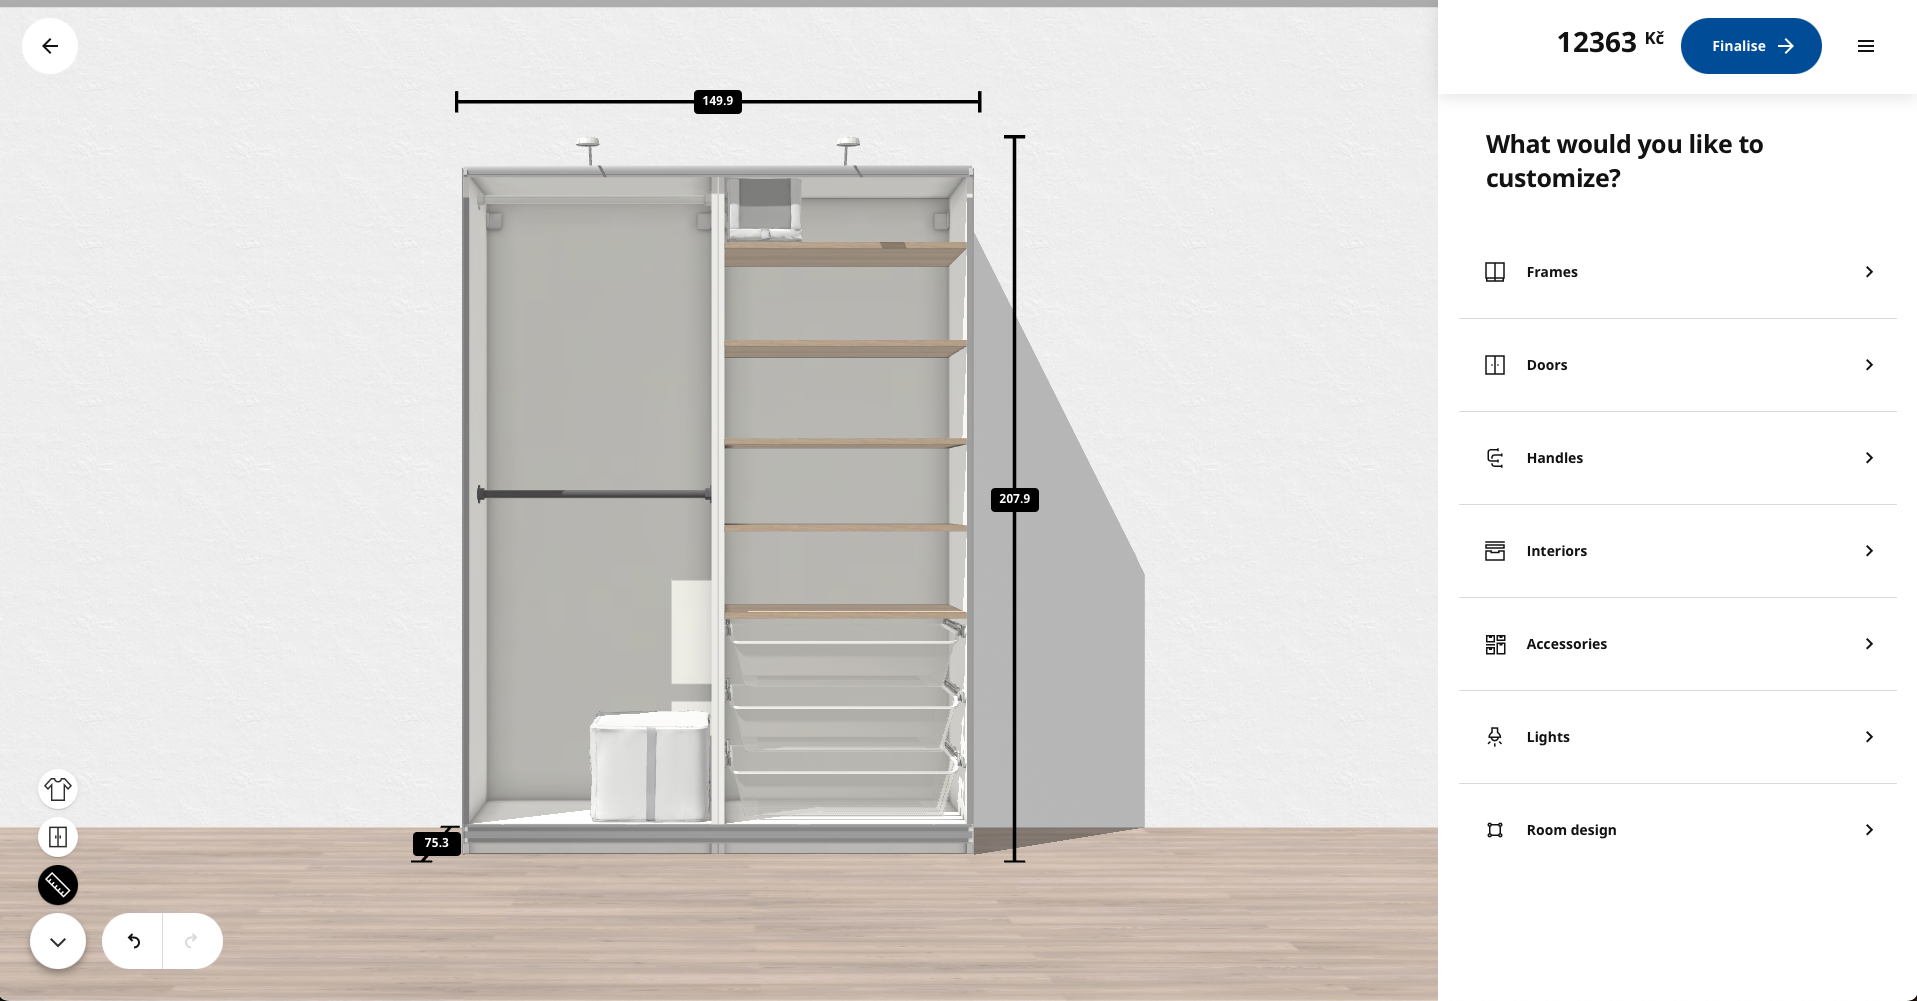
\includegraphics[width=\textwidth]{images/analysis_ikea-pax.png}
\caption{Screenshot of IKEA PAX Planner Tool with example configuration}
\end{figure}

The tool consists mainly of two views. The primary view on the left contains a 3D preview of the configured product, allowing users to observe objects from different viewpoints by moving along an orbital trajectory in a 180\textdegree half-circle. The components displayed in the 3D view are both realistic and interactive. Users can adjust their position by dragging, and selecting a component offers additional information and real-life images of the item. All modular options that can be added to the current configuration are found in the secondary smaller view on the right side and can be added by clicking or dragging them into the 3D preview. The application is responsive, and on mobile devices, the secondary view moves from the right side to a bottom sliding panel. The navigation bar is located at the top of the secondary view, and other buttons are located around the edges of the primary view.

At the beginning of the configuration process, the application prompts the user to select the starting point of the configuration. The configurator has open navigation, meaning that the components can then be configured in any order. Components can be placed anywhere along a specified axis within certain restrictions, effectively preventing the creation of impossible configurations.

The tool performs live price calculations and contains a final summary confirmation screen from which it is possible to order the configured product in the e-shop. The configurator maintains a history of recent changes, accessible through undo and redo buttons. It also features the ability to save configurations on the server, which can be retrieved later using a generated code.

The app is a single-page application (SPA is a web application implementation approach that loads only a single page and then sequentially updates the content of the page with scripting on the client side, rather than loading whole new pages from the server \cite{Fink2014}) and does not update the URL based on the selected product or phase of the configuration.

The configurator also provides a range of innovative features, such as the ability to change the visibility of some elements using a button (hiding the doors of a wardrobe to reveal the contents inside) or the ability to display dimensions directly in the 3D view.


%______________________________________________________________
\subsubsection{Muuto Product Planner}

Muuto is a Scandinavian design company that produces furniture and home accessories. \cite{Muuto}

The company provides Product Planner, a 3D web-based configurator, which allows customers to customize and combine the designs of various products, such as storage systems, sofas, tables, or wall hangers, tailored to their specific needs. \footnote{Available at: \url{https://planner.muuto.com/}}

\begin{figure}[h]
\centering
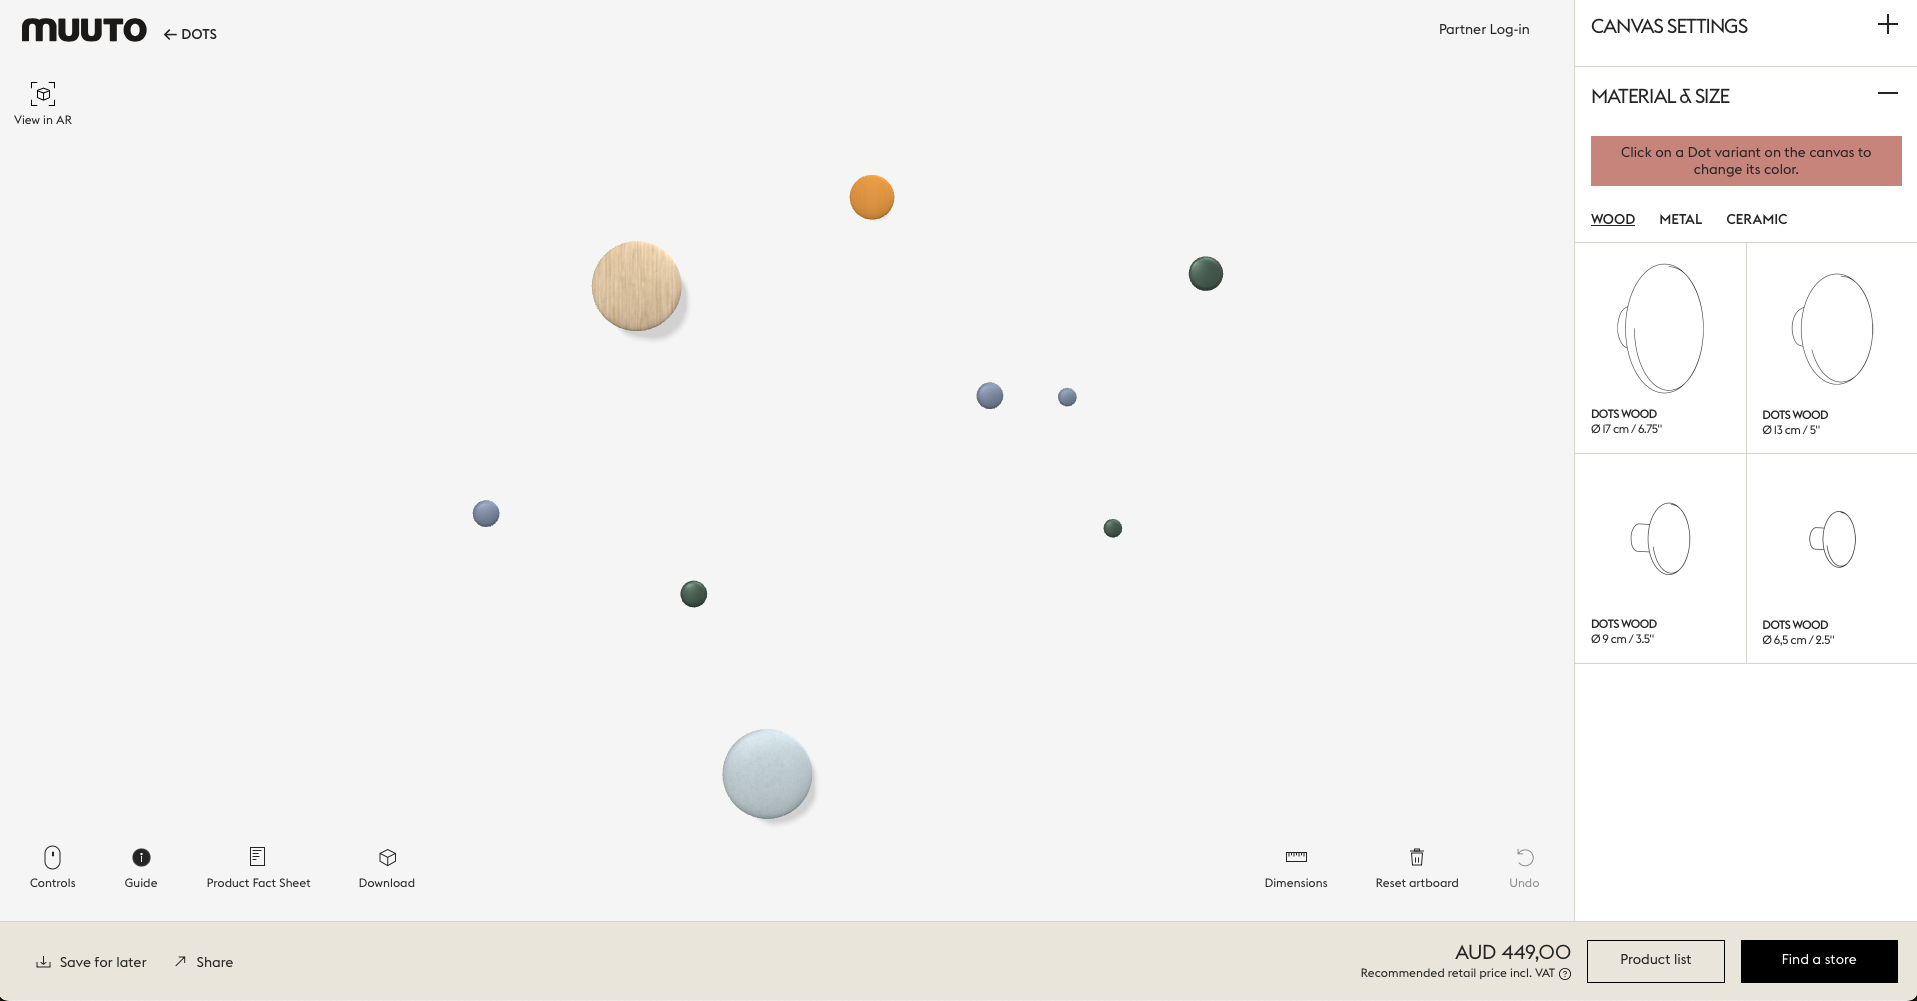
\includegraphics[width=\textwidth]{images/analysis_muuto-product-planner.png}
\caption{Screenshot of Muuto Product Planner tool with example configuration}
\end{figure}

The design of the configurator is similar to that in the previous case. The configurator also consists of two views. The primary view on the left provides full realistic 3D visualization, while the smaller secondary view on the right side allows users to add components by dragging them into the main view. Selecting a component in the primary view enables users to remove it or alter its materials. As the design is responsive, on smaller devices, the secondary view transforms into a bottom slide panel. Depending on the configured product, the tool offers a preview from a single angle or a preview from any point on an orbital trajectory. The main view is also surrounded by buttons along its edges. The navigation bar is positioned at the bottom across the entire application, while the company logo is displayed on the top left.

The tool follows a similar flow, starting with the selection of the starting point and then moving to the configurator process, which has open navigation. Components can be placed anywhere, unless their position is dependent on another component. Due to this flexibility and also the wide variety of products that it supports, the configurator is not restricted to generating configurations that are feasible to produce and can create impossible configurations.

The tool can display real dimensions and can reverse the performed changes using the undo and redo button. The configuration can also be saved on the server side and later accessed using a unique code. Live price calculation is also performed, and there is a summary page, but it is not possible to order the configured product; instead, the user is redirected to a physical store locator.

Furthermore, the designed configuration can be quickly shared with other users using email, or it can be downloaded in several file formats containing the 3D model itself. The application makes it possible to view the product in AR, directly in a web browser, albeit only on Apple devices using the Universal Scene Description (USDZ) format and AR~Quick Look. \cite{Jackson2018}

The application has multiple URL schemes that depend on the configuration phase, but they are not determined by the current product. 

%______________________________________________________________
\subsubsection{LD Seating Nido Configurator}

LD Seating is a company based in the Czech Republic that specializes in the production of chairs, armchairs, and sofas. \cite{LDSeating}

The company uses a 3D web-based configurator to market the Nido modular seating system, which consists of elements that are designed to be combined in various ways. \footnote{Available at: \url{https://nido.ldseating.com/en/configurator}}

\begin{figure}[ht]
\centering
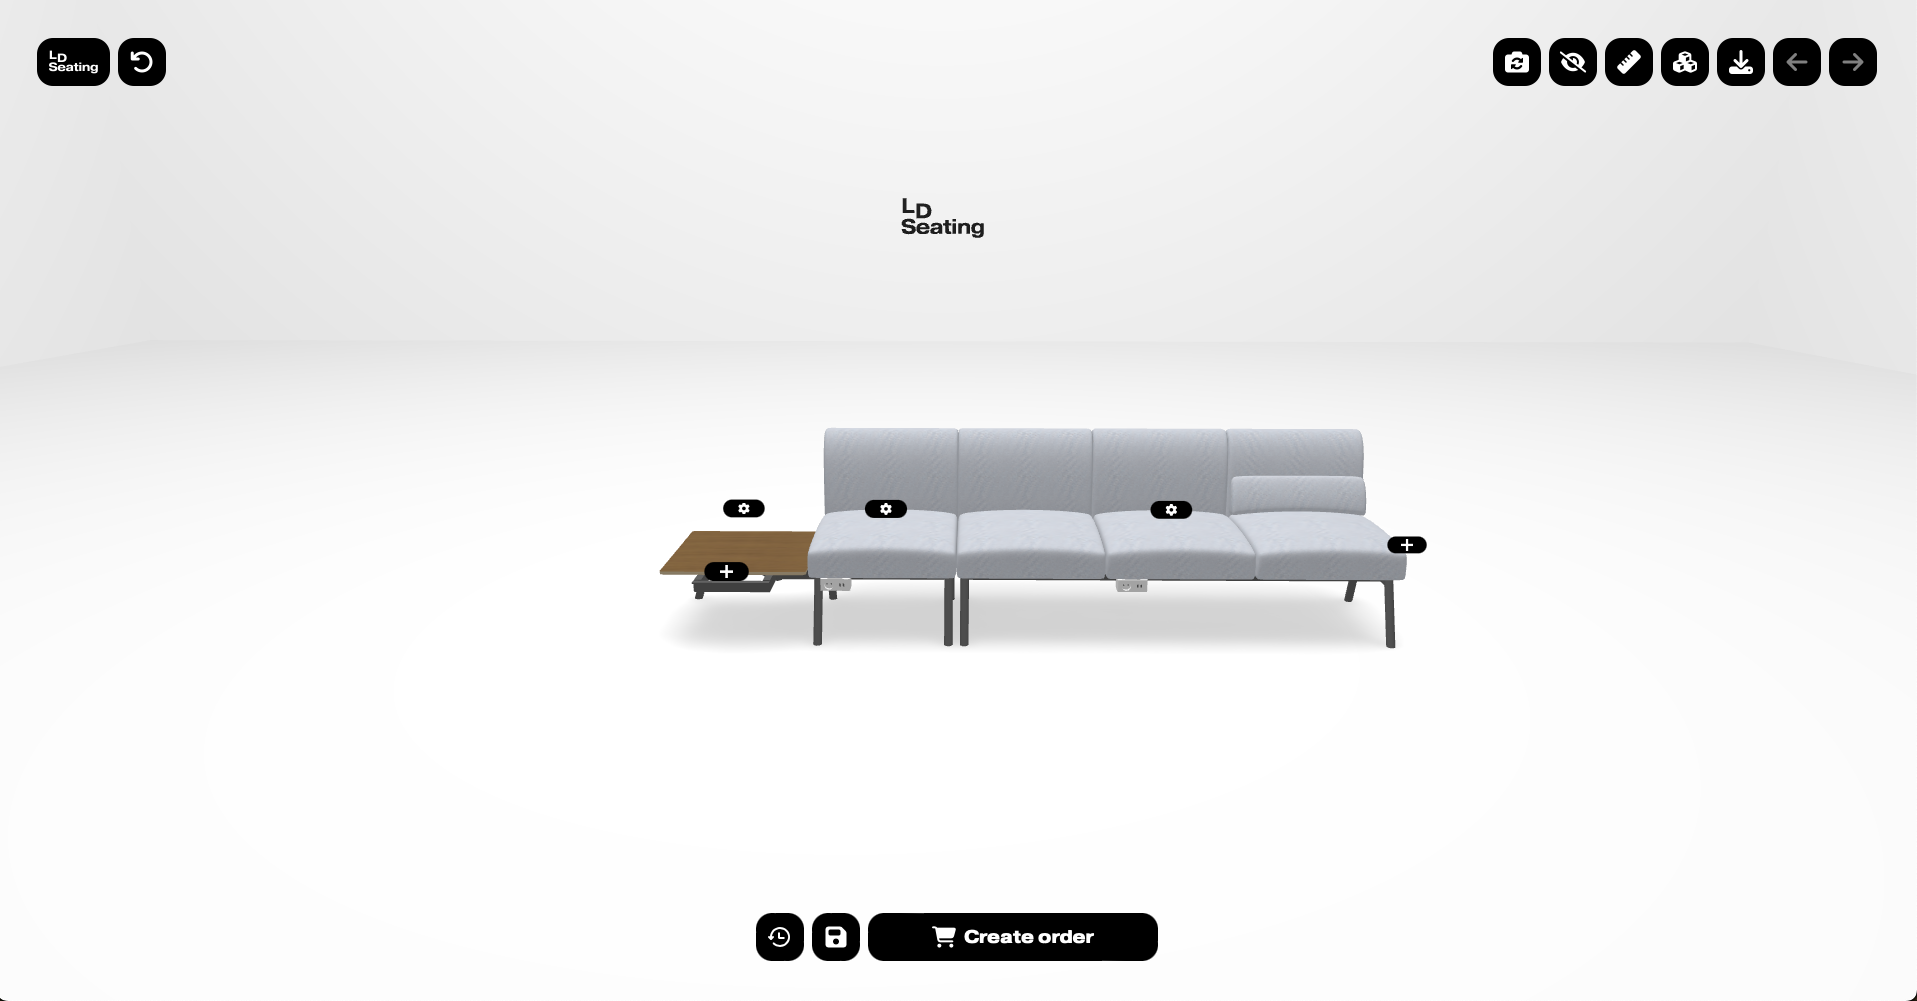
\includegraphics[width=\textwidth]{images/analysis_nido-configurator.png}
\caption{Screenshot of LD Seating Nido Configurator with example configuration}
\end{figure}

The configurator consists of one large view, covering the whole application, which displays high-definition 3D models of the configured components. The buttons are placed around the entire view, on the top right, bottom center, and top left, where the company logo is also displayed.  The controls for adding components and modifying properties are embedded directly in the 3D scene. When necessary, a panel opens to the right, allowing users to select components to add, adjust component properties, or change materials. The application is partially responsive, as the side panel opens fullscreen on smaller viewports; however, there are some issues with image and text overflows on mobile devices. The main view allows the user to observe the configuration from all angles along an orbital trajectory.

The flow of the application also includes selecting a starting point. The product configuration process itself uses open navigation. The tool assesses whether a component can fit into a space and, if not, prevents its placement, thereby restricting impossible configurations. At the completion of the configuration, a confirmation summary is presented; however, in this case, the price is not calculated live; therefore, the configurator cannot directly place an order for the product, but instead pressing the configuration confirmation results in the display of an inquiry form.

The resulting configuration can be downloaded as a file with a 3D model. The configuration can also be saved server-side, which generates a unique link on which the configuration is accessible. The tool features a version history that stores each saved configuration for future access. Users can revisit these versions later, with undo and redo buttons also available. The resulting configuration can also be exported to a PDF file containing a list of components. The tool also has the ability to display dimensions.

The application is an SPA, maintaining a consistent URL or changing it to reflect the location of a saved configuration if one exists.


% - - - - - - - - - - - - - - - - - - - - - - - - - - - - - - -
\subsection{Available toolkits}
% - - - - - - - - - - - - - - - - - - - - - - - - - - - - - - -

In this section of the analysis chapter, the focus shifts from specific 3D modular configurator applications to the fundamental toolkits that power the configurators. Although many configurators are bespoke and tailored to the specific needs of companies and their individual products, there are providers offering more generic and adaptable solutions. These offerings are highly relevant to this thesis, as the objective of this thesis is to create a product-agnostic toolkit, which means that there is a need to consider the way the configurator is set up by the business.

A variety of providers offer these toolkits for creating product configurators, intending to provide semi-custom or fully custom solutions, as well as generic options. This section examines two particular toolkits to carry out a focused and relevant analysis. The choice of toolkits analyzed has been complicated by the fact that most providers are quite cautious about the details of the technology, typically revealing in-depth information only after a serious business inquiry. The choice was also based on factors such as the implementation approach and compatibility with modular products.

\noindent This section seeks to answer the following questions about the toolkits: 
\begin{itemize}[label=\rectanglebullet]
    \item \textbf{Administration}: How is the product configurator created and administered?
    \item \textbf{Assets}: How are assets stored and cataloged?
    \item \textbf{Product configuration}: How are the configuration options and rules defined?
    \item \textbf{Integration}: How is the tool integrated into other systems?
    \item \textbf{Pricing}: What is the cost of the offered solution?
\end{itemize}
%______________________________________________________________
\subsubsection{Threekit}

Threekit is a leading global company in visual commerce technologies that specializes in 3D product visualizations. The Threekit Platform, which enables clients to configure interactive product experiences according to their needs, functions as an administrative application and has the capability to generate product configurators (see \autoref{fig:threekit-platform}). \cite{ThreeKitAboutUs} \cite{ThreeKitPlatform}

The platform is very complex with many distinct features. At its core, it uses a catalog for storing all product data (the products themselves, materials used, configurable parts, etc.). The items in the catalog can then be loaded into The Treekit Player, which will display the models in 3D, with the option for users to change attributes (models and materials) that are tied to the item. The behavior of the configurator can be set up using item rules and logic that support conditions, queries, and even custom scripts. The platform also offers a data tables feature that is similar to spreadsheets and is designed to handle extensive configuration data and logic. The application also has a built-in asset editor for refining 2D and 3D assets and configuration options (see \autoref{fig:threekit-editor}). Models of the products can be uploaded in many 3D formats. The platform provides API integration with the leading e-Commerce and ERP systems. \cite{ThreeKitPlatformDocumentation}

The offered solution is still partially tailored to the client, which is the reason why the service does not have standardized pricing. Instead, the price is determined through a personalized quote. It is important to note that the analysis of Threekit presented here is based on the publicly available documentation of the platform. Direct access to the full suite of Threekit's tools is typically available only after formalizing a business agreement with the company.


%______________________________________________________________
\subsubsection{Roomle}

Roomle is an Austrian company focused on pioneering visual product configuration. They provide solutions for product visualization, room design, and product configurators. Roomle's solution, called Rubens, is the \enquote{Open Full Logic 3D-Configurator}. The tool utilizes both parametric and modular mechanisms. The software allows integration with third parties through the use of an API. In addition, it supports front-end technologies on web and mobile platforms and has a built-in AR experience. \cite{RoomleAbout}

Web application, Rubens Admin, is used to set up the configurator application. To add a product which will then be configured by customers, 3D models and materials are uploaded to the admin application. Components are defined using the RoomleScript language, which is loosely based on the JavaScript language. The design of the configurator itself can be tuned in the admin application as well. Multiple language variants can be defined for product names and descriptions. The configurator application (see \autoref{fig:roomle}) runs on the client side and can be simply embedded into a website. Additionally, it can utilize a JavaScript library that can subscribe to events or modify the configurator. A framework is also provided to utilize the configurator within an iOS application. \cite{RoomleDocumentation}

In terms of pricing, Roomle's Rubens configurator with the listed capabilities is offered to businesses at a monthly fee of €1450. \cite{RoomleFullLogic}

% - - - - - - - - - - - - - - - - - - - - - - - - - - - - - - -
\subsection{Summary of existing solutions analysis}
% - - - - - - - - - - - - - - - - - - - - - - - - - - - - - - -

All the product configurators analyzed have common characteristics, especially in terms of navigation and visualization styles, which remain consistent across different tools. Despite this, certain trade-offs were observed between them, especially regarding placement options. While some solutions offer users the freedom to position components anywhere, others restricted placement to fixed points. This variance stems from implementation complexity, as the fixed-point system is simpler, furthermore offering a better way to restrict impossible configurations.
Another significant distinction was observed in the product finalization process, which ranged from the ability to place an order to being directed to a physical store.

The key points discussed in the analysis of modular product configurators are summarized in the following table (see \autoref{table:summary-analysis}).

\begin{table}[ht!]
\centering
\begin{tabular}{>{\raggedright\arraybackslash}p{3.8cm}*{3}{>{\centering\arraybackslash}p{2.5cm}}} 
\toprule
\parbox[c][7ex]{3.8cm}{\textbf{Features}} &
\multrow{c}{\textbf{IKEA} \\ \textbf{Pax} \\ \textbf{Planner}} &
\multrow{c}{\textbf{Muuto} \\ \textbf{Product} \\ \textbf{Planner}} &\multrow{c}{\textbf{LD Seating} \\ \textbf{Nido} \\ \textbf{Configurator}} \\ 
\midrule
\parbox[c][7ex]{3.8cm}{Navigation}
    & Open
    & Open
    & Open \\ 
\parbox[c][7ex]{3.8cm}{Visualization}
    & Realistic
    & Realistic
    & Realistic \\ 
\parbox[c][7ex]{3.8cm}{Placement options}
    & Free
    & Free
    & Fixed points\\ 
\parbox[c][7ex]{3.8cm}{Camera movement}
    & Orbital
    & \multrow{c}{Orbital; \\ Static}
    & Orbital \\
\parbox[c][7ex]{3.8cm}{Impossible \\ configurations} 
    & No
    & Yes
    & No \\
\parbox[c][7ex]{3.8cm}{Responsiveness}
    & Yes
    & Yes
    & Yes \\
\parbox[c][7ex]{3.8cm}{Price calculation}
    & Yes
    & Yes
    & No \\
\parbox[c][7ex]{3.8cm}{Purchase option}
    & E-shop order
    & Store locator
    & Inquiry form \\
\parbox[c][7ex]{3.8cm}{Save option}
    & Server-side
    & \multrow{c}{Server-side; \\ Local}
    & \multrow{c}{Server-side; \\ Local} \\
\parbox[c][7ex]{3.8cm}{Version history}
    & Undo \& redo 
    & Undo \& redo
    & \multrow{c}{Undo \& redo; \\ Multiple saves} \\
\parbox[c][7ex]{3.8cm}{VR or AR}
    & No
    & Yes
    & No \\
\bottomrule
\end{tabular}
\caption{Summary of key points discussed in the analysis of modular product configurators}
\label{table:summary-analysis}
\end{table}


The user interface design of the analyzed configurations also displayed similarities, particularly in layout style, featuring a primary 3D preview on the left, a secondary view on the right, and buttons surrounding the primary view.

Analyzing the offered toolkit solutions proved challenging due to the information being closely guarded, as it is in the financial interest of the providers. However, the examined toolkits are very sophisticated solutions that are supported by large backend services, which are used for storing assets and facilitating the configurators functionality. The toolkits offer advanced features that allow for the definition of rules and logic, allowing companies to create configurators with a large amount of complexity. This indicates that these toolkits target a market composed mainly of larger corporations that require sophisticated solutions, which is also reflected in pricing.

%---------------------------------------------------------------
\section{Proposed solution}
%---------------------------------------------------------------

This thesis aims to develop a new solution for the configuration of modular products. To do so, the proposed solution will incorporate the common characteristics identified in the analyzed solutions. The following chapter outlines the features that should be implemented in the solution proposed in this thesis.

The main differentiation factor of this proposed toolkit is its emphasis on catering to small businesses. As the existing toolkits that were examined were costly and mainly aimed at larger companies, this solution aims to fill this market gap. To achieve this, it will be necessary to make some trade-offs, ensuring the solution's adaptability and relevance across various product types without making the solution overly complex. Therefore, the proposed toolkit will prioritize simplicity and cost-effectiveness, following the best practices seen in larger-scale solutions but with a specific focus on the needs and capabilities of the target market.
 
The proposed toolkit is envisioned to be universal with regard to products, adaptable, and customizable, catering to a wide variety of modular products and industries. The solution should be simple for businesses to deploy and manage, without the need for extensive technical resources, ensuring that it is straightforward for smaller businesses to maintain and operate effectively.

% - - - - - - - - - - - - - - - - - - - - - - - - - - - - - - -
\subsection{Requirement engineering} \label{requirements}
% - - - - - - - - - - - - - - - - - - - - - - - - - - - - - - -

Following the overview of objectives and the definition of the target market, it is necessary to formulate precise requirements for this solution. Detailing these features and characteristics is crucial for successful implementation. Thus, the description of requirements engineering for this solution will be provided here.

The process of requirements engineering for software products involves gathering, analyzing, selecting, and managing requirements. It focuses on interpreting and understanding the goals, needs, and beliefs of stakeholders and transforming them into specific requirements.
Software requirements can be separated into two categories: \cite{Aurum2005}
\begin{enumerate}
    \item Functional requirements: These requirements describe what the system should be able to do. They specifically outline the system's behavior and its interactions in specific situations.
    \item Non-functional requirements: These requirements put constraints on the solution that meets the functional requirements, rather than being focused on specific behaviors of the system. They are often, among others, focused on performance, security, accessibility, and compatibility.
\end{enumerate}

To manage and prioritize these requirements, each is assigned an approximate priority level using the MoSCoW method. This approach classifies the requirements into four distinct categories: \cite{Kravchenko2022}
\begin{enumerate}
    \item Must: Requirements crucial for the final solution.
    \item Should: Requirements to be implemented if feasible.
    \item Could: Desirable but not essential requirements.
    \item Won't: Nice-to-have requirements that most likely are not going to implemented in this solution.
\end{enumerate}
This method helps to plan and allocate resources throughout the implementation phase.

Additionally, each requirement is given a rough estimate of the implementation difficulty, separated into three categories:
\begin{enumerate}
    \item Simple: Requirements that are straightforward to implement and require few resources, time, or technical challenges.
    \item Intermediate: Requirements that pose moderate challenges and demand a considerable amount of resources, time, and problem-solving.
    \item Complex: Requirements that are extremely challenging and involve substantial resources, time, and expertise.
\end{enumerate}
This preliminary assessment aims to classify the requirements without relying on specific rigid criteria for each category. This method is specifically used only for functional requirements, as non-functional requirements affect the software's functionality and user experience through abstract constraints, making them unsuitable for the same difficulty estimation approach.
% - - - - - - - - - - - - - - - - - - - - - - - - - - - - - - -
\subsubsection{Functional requirements}
% - - - - - - - - - - - - - - - - - - - - - - - - - - - - - - -

\begin{enumerate}
\item \textbf{F1:} \label{itm:F1} 3D product visualization
\vspace{2pt}
\\The tool shall offer users 3D visualization of their configured product, employing realistic models to accurately represent the components used and their characteristics.
\begin{description}[noitemsep]
    \item[Priority:] Must
    \item[Difficulty:] Complex
\end{description}
\vspace{4pt}

\item \textbf{F2:} \label{itm:F2} Dynamic orbital camera controls
\vspace{2pt}
\\The tool should have dynamic orbital camera controls that allow users to view the product in 3D product visualization (see requirement \hyperref[itm:F1]{F1}) from any angle by rotating, panning, and zooming the camera around the product. This feature aims to provide an engaging visual experience that allows users to examine the product with a 360-degree view. Controls should be intuitive, allowing seamless navigation through mouse actions or touch gestures depending on the device being used.
\begin{description}[noitemsep]
    \item[Priority:] Must
    \item[Difficulty:] Simple
\end{description}
\vspace{4pt}

\item \textbf{F3:} \label{itm:F3} Modularity configuration mechanism
\vspace{2pt}
\\The toolkit should incorporate modularity mechanisms that allow users to configure products by adding, removing or modifying components within the overall product or in relation to other components. Different versions may be available for each component, and the toolkit administrator should have the ability to designate them either as optional or mandatory, thereby enhancing the flexibility of configuration.
\begin{description}[noitemsep]
    \item[Priority:] Must
    \item[Difficulty:] Intermediate
\end{description}
\vspace{4pt}

\item \textbf{F4:} \label{itm:F4} Component interactivity
\vspace{2pt}
\\The configurator should support interactivity with each component of the product. Users should be able to select components directly within the 3D visualization (see requirement \hyperref[itm:F1]{F1}), which should allow them to change attributes of the components, remove it or swap it with alternative options (see requirement \hyperref[itm:F3]{F3}). The changes made by the users should be immediately visible, allowing for an iterative and engaging customization process. Moreover, the components that are interacted with need to offer feedback, such as highlighting, in order to assist users in navigating the accessible customization choices.
\begin{description}[noitemsep]
    \item[Priority:] Should
    \item[Difficulty:] Complex
\end{description}
\vspace{4pt}

\item \textbf{F5:} Open navigation
\vspace{2pt}
\\The configurator should offer high flexibility in the order of configuring components and attributes, avoiding a linear step-by-step configuration and requiring all changes to be performed at any point during the configuration process. This flexibility enhances the user's ability to navigate freely among various different components of the product (see requirement \hyperref[itm:F3]{F3}).
\begin{description}[noitemsep]
    \item[Priority:] Should
    \item[Difficulty:] Simple
\end{description}
\vspace{4pt}

\item \textbf{F6:} \label{itm:F6} Fixed point component placement
\vspace{2pt}
\\In alignment with the modularity configuration mechanism (see requirement \hyperref[itm:F3]{F3}), the configurator should enable components to be attached to other components or the main product exclusively at predefined fixed points. While this approach restricts the potential solution space, it greatly streamlines the configuration process from the user side and helps to ensure that the configured product remains within the realm of feasible configurations.
\begin{description}[noitemsep]
    \item[Priority:] Should
    \item[Difficulty:] Intermediate
\end{description}
\vspace{4pt}

\item \textbf{F7:} \label{itm:F7} Component collision detection
\vspace{2pt}
\\The tool should incorporate a collision detection system to prevent components from being positioned in such a way that would result in physical overlaps during configuration. This feature is essential to maintain the realism and feasibility of the configured product.
\begin{description}[noitemsep]
    \item[Priority:] Could
    \item[Difficulty:] Complex
\end{description}
\vspace{4pt}

\item \textbf{F8:} \label{itm:F8} Material color configuration
\vspace{2pt}
\\Users should be able to modify the appearance of components and products through a selection from a palette of materials and colors, predefined by the toolkit's administrator. The chosen appearance should immediately be reflected in the 3D visualization (see requirement \hyperref[itm:F1]{F1}) of the configuration.
\begin{description}[noitemsep]
    \item[Priority:] Could
    \item[Difficulty:] Complex
\end{description}
\vspace{4pt}

\item \textbf{F9:} \label{itm:F9} Configuration review
\vspace{2pt}
\\Before the configuration process is finalized, users should be presented with a review page that allows for a detailed examination of their product configuration. This feature should provide a summary listing all selected components, materials, colors, and any custom parameters. In addition, users should be able to return to previous configuration steps to make any necessary adjustments.
\begin{description}[noitemsep]
    \item[Priority:] Should
    \item[Difficulty:] Simple
\end{description}
\vspace{4pt}

\item \textbf{F10:} \label{itm:F10} Configuration confirmation
\vspace{2pt}
\\At the end of the configuration process, users should be presented with a confirmation button, provided that an administrator has set up a specific confirmation action for the product. This button is intended for users to confirm their choices and trigger a predetermined action, like performing an API request or being directed to another page, as specified by the administrator. This should allow for a smooth transition, where, upon configuration confirmation, the user is engaged in a follow-up action, like a checkout process or being guided to a physical store locator page. The ability to perform a custom API call set by the administrator at the end of the configuration process provides a flexible way to integrate the configurator with different systems or processes, thus improving its functionality and delivering a seamless user experience from start to finish.
\begin{description}[noitemsep]
    \item[Priority:] Should
    \item[Difficulty:] Simple
\end{description}
\vspace{4pt}

\item \textbf{F11:} Inquiry form \label{itm:F11}
\vspace{2pt}
\\As an extension of configuration confirmation (see requirement \hyperref[itm:F10]{F10}), the administrator should be able to set the product's confirmation action to trigger an inquiry form. In this scenario, when users click on the confirmation button, they should encounter a form asking for their contact details. Once completed, the created product configuration along with the user's contact information should be sent to an API predefined by the toolkit's administrator. This allows for a standard inquiry form process directly within the configurator application.
\begin{description}[noitemsep]
    \item[Priority:] Should
    \item[Difficulty:] Simple
\end{description}
\vspace{4pt}

\item \textbf{F12:} Configuration local saving and retrieval
\vspace{2pt}
\\The tool should allow users to save the current product configuration locally, allowing them to pause the customization process without losing progress. Users should have the ability to easily access and resume editing their saved configurations at a later time. The advantage of local save functionality compared to server-side saves is that it requires no active management or intervention from the toolkit operator, simplifying the system's overall maintenance.
\begin{description}[noitemsep]
    \item[Priority:] Could
    \item[Difficulty:] Intermediate
\end{description}
\vspace{4pt}

\item \textbf{F13:} \label{itm:F13} Undo and redo actions
\vspace{2pt}
\\The configurator should integrate undo and redo functionality, enabling users to easily revert or reapply changes made anytime during the configuration process.
\begin{description}[noitemsep]
    \item[Priority:] Should
    \item[Difficulty:] Intermediate
\end{description}
\vspace{4pt}

\item \textbf{F14:} Interface color scheme customization \label{itm:F14}
\vspace{2pt}
\\The interface of the configurator should offer customizable options, enabling the toolkit's administrator to tailor the color scheme and images to align with the branding and design of the business using the toolkit.
\begin{description}[noitemsep]
    \item[Priority:] Could
    \item[Difficulty:] Simple
\end{description}
\vspace{4pt}

\item \textbf{F15:} \label{itm:F15} Interface texts customization
\vspace{2pt}
\\The toolkit should provide a way for the administrator to change the textual contents of the configurator's interface, ensuring that the language, tone, and terminology used are perfectly aligned with the business's needs and reflect the business's terminology and branding.
\begin{description}[noitemsep]
    \item[Priority:] Could
    \item[Difficulty:] Intermediate
\end{description}
\vspace{4pt}

\item \textbf{F16:} \label{itm:F16} Visual product catalog management
\vspace{2pt}
\\The toolkit should provide administrators with the ability to visually manage the catalog of configurable products and their components. The visual preview of the components provided within catalog management should mirror the 3D previews in the actual configuration process (see requirement \hyperref[itm:F1]{F1}). This management system should allow administrators to add, update, or remove products and components, along with specifying their precise mounting locations, directly through an intuitive visual interface (see requirement \hyperref[itm:F6]{F6}).
\begin{description}[noitemsep]
    \item[Priority:] Must
    \item[Difficulty:] Complex
\end{description}
\vspace{4pt}

\item \textbf{F17:} Product properties and attributes management
\vspace{2pt}
\\The toolkit should provide a way to manage the properties and attributes of the products and components in the catalog (see requirement \hyperref[itm:F16]{F16}), allowing administrators to define and adjust the characteristics that users can configure. It should allow for the detailed specification of each product's features, such as color options, material types (see requirement \hyperref[itm:F8]{F8}), and any other attributes that define the product's functionality and appearance.
\begin{description}[noitemsep]
    \item[Priority:] Must
    \item[Difficulty:] Complex
\end{description}
\vspace{4pt}


\item \textbf{F18:} Real-time price calculation
\vspace{2pt}
\\If the configured attributes and components have prices predefined by the toolkit's administrator, the configurator should automatically update and display the price of the whole customized product with every change made. The tool should be capable of dealing with different currencies.
\begin{description}[noitemsep]
    \item[Priority:] Won't
    \item[Difficulty:] Intermediate
\end{description}
\vspace{4pt}

\item \textbf{F19:} AR viewing capabilities
\vspace{2pt}
\\The configurator should extend its visualization features (see requirement \hyperref[itm:F1]{F1}) to include AR viewing capabilities, enabling users to project their configured products into their real-world environment through their device's camera. In case the device they are using does not have AR capability, the tool should provide a seamless way for the user to open the configuration in AR on another device that does have such capability.
\begin{description}[noitemsep]
    \item[Priority:] Won't
    \item[Difficulty:] Complex
\end{description}
\vspace{4pt}

\end{enumerate}


% - - - - - - - - - - - - - - - - - - - - - - - - - - - - - - -
\subsubsection{Non-functional requirements}
% - - - - - - - - - - - - - - - - - - - - - - - - - - - - - - -

\begin{enumerate}

\item \textbf{NF1:}\label{itm:NF1} Multiplatform compatibility
\vspace{2pt}
\\The solution should work smoothly on various operating systems and devices, such as desktop and mobile platforms, to ensure broad accessibility. This ensures that the solution is accessible to a wide audience, regardless of their preferred technology, thereby maximizing user engagement and reach.
\begin{description}
    \item[Priority:] Must
\end{description}
\vspace{4pt}

\item \textbf{NF2:}\label{itm:NF2} Responsiveness
\vspace{2pt}
\\The user interface should be responsive, adapting to viewport sizes and resolutions on different screens, ensuring an optimal viewing and interaction experience across all supported devices.
\begin{description}
    \item[Priority:] Must
\end{description}
\vspace{4pt}

\item \textbf{NF7:} Self-hostable architecture
\vspace{2pt}
\\The toolkit should be designed with the intent of being deployed and hosted on a business's preferred infrastructure, whether on-premises or in a private cloud. This facilitates greater control over the data and security according to the operator's policy, as well as flexibility for possible modifications.
\begin{description}
    \item[Priority:] Must
\end{description}
\vspace{4pt}

\item \textbf{NF4:} Infrastructure
\vspace{2pt}
\\The toolkit should ideally operate on the existing infrastructure of the business, leveraging the resources that may already be used to offer the products. The configurator application is expected to operate primarily on the client side, requiring only minimal back-end support, possibly making use of a simple serverless architecture if needed. This approach reduces the demand for maintenance and is cost effective, improving existing operations without necessitating significant new investments in infrastructure.
\begin{description}
    \item[Priority:] Must
\end{description}
\vspace{4pt}

\item \textbf{NF5:} \label{itm:NF5} Maintainability
\vspace{2pt}
\\The codebase and architecture should be designed to facilitate easy maintenance, straightforward updates, modifications, and enhancements. To ensure that the toolkit remains robust and flexible for future needs, industry standards and best practices should be adhered to during implementation. The tool should require minimal routine maintenance by the administrator.
\begin{description}
    \item[Priority:] Must
\end{description}
\vspace{4pt}

\item \textbf{NF6:} Documentation
\vspace{2pt}
\\To support maintainability (see requirement \hyperref[itm:NF5]{NF5}) and ease of use, comprehensive documentation is essential. This should cover the configurator's setup, deployment, customization options, and guides on managing products, components, and user interactions. Providing comprehensive and detailed documentation guarantees that administrators and developers can efficiently employ and customize the configurator to suit their individual requirements. It serves as a valuable resource for troubleshooting, further development, and maximizing the potential of the tool.
\begin{description}
    \item[Priority:] Should
\end{description}
\vspace{4pt}

\item \textbf{NF7:} Performance
\vspace{2pt}
\\The toolkit should ensure optimal performance under typical usage load, with swift loading and quick response times across all compatible devices, particularly those with lower processing power.
\begin{description}
    \item[Priority:] Must
\end{description}
\vspace{4pt}

\item \textbf{NF8:} \label{itm:NF8} Multilingual support
\vspace{2pt}
\\The configurator should offer multilingual support. Administrators should be able to simply add, remove, or update languages, thus making it easier to adapt the interface for different language versions. This capability builds on the interface text customization requirement (see requirement \hyperref[itm:F15]{F15}), extending its scope to include different language options. Users should be provided with a simple method to select their preferred language.
\begin{description}
    \item[Priority:] Could
\end{description}
\vspace{4pt}

\end{enumerate}